\documentclass[border=8pt]{standalone}
\usepackage{pgfplots}
\pgfplotsset{compat=1.18, trig format plots=deg}
\begin{document}
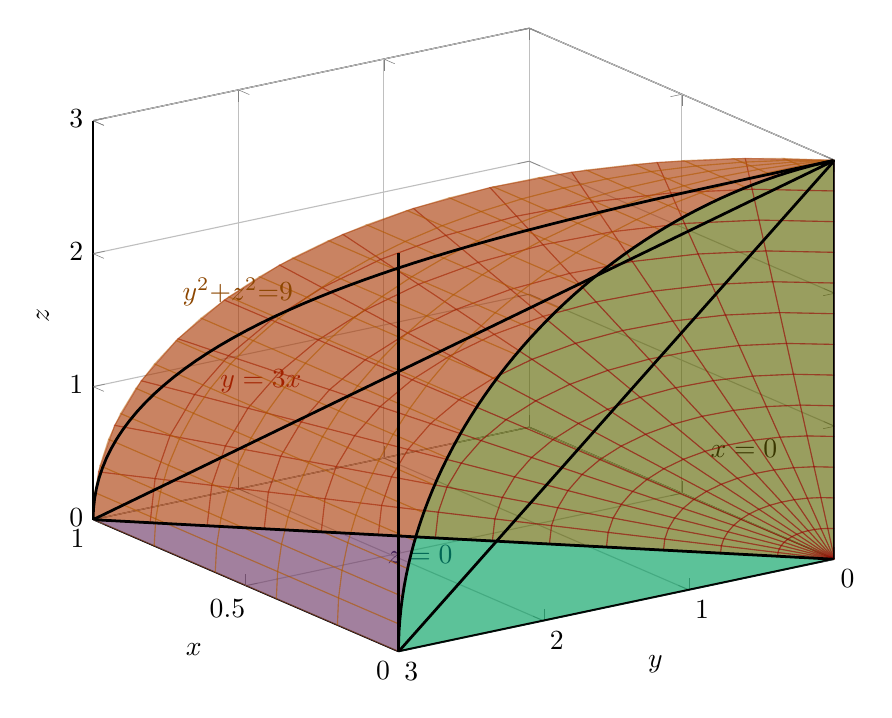
\begin{tikzpicture}
\begin{axis}[
    width=11cm, height=9.5cm,
    view={-125}{22},
    xlabel={$x$}, ylabel={$y$}, zlabel={$z$},
    xmin=0,xmax=1, ymin=0,ymax=3, zmin=0,zmax=3,
    xtick={0,0.5,1}, ytick={0,1,2,3}, ztick={0,1,2,3},
    grid=major,
]
% ---- face z = 0 : triangle (0,0)-(0,3)-(1,3) ----
\addplot3[fill=blue, opacity=0.40, draw=black, line width=0.7pt]
  coordinates {(0,0,0) (0,3,0) (1,3,0) (0,0,0)};
\node[blue!55!black, font=\bfseries] at (axis cs:0.62,1.55,-0.22) {$z=0$};

% ---- face x = 0 : quarter disk in the yz-plane ----
\addplot3[fill=green, opacity=0.40, draw=none] coordinates {
(0,0,0) (0,3.0000,0.0000) (0,2.9959,0.1570) (0,2.9836,0.3136)
 (0,2.9631,0.4693) (0,2.9344,0.6237) (0,2.8978,0.7765)
 (0,2.8532,0.9271) (0,2.8007,1.0751) (0,2.7406,1.2202)
 (0,2.6730,1.3620) (0,2.5981,1.5000) (0,2.5160,1.6339)
 (0,2.4271,1.7634) (0,2.3314,1.8880) (0,2.2294,2.0074)
 (0,2.1213,2.1213) (0,2.0074,2.2294) (0,1.8880,2.3314)
 (0,1.7634,2.4271) (0,1.6339,2.5160) (0,1.5000,2.5981)
 (0,1.3620,2.6730) (0,1.2202,2.7406) (0,1.0751,2.8007)
 (0,0.9271,2.8532) (0,0.7765,2.8978) (0,0.6237,2.9344)
 (0,0.4693,2.9631) (0,0.3136,2.9836) (0,0.1570,2.9959)
 (0,0.0000,3.0000) (0,0,0)};
\node[green!35!black, font=\bfseries] at (axis cs:-0.25,1.15,1.35) {$x=0$};

% ---- face y = 3x  (i.e. x = y/3), ruled over the quarter disk ----
\addplot3[surf, domain=0:3, y domain=0:90, samples=14, samples y=14,
          opacity=0.38, shader=flat, color=red!60!black]
  ({(x*cos(y))/3}, {x*cos(y)}, {x*sin(y)});
\node[red!60!black, font=\bfseries] at (axis cs:0.95,1.95,0.85) {$y=3x$};

% ---- cylindrical face y^2+z^2 = 9 , 0 <= x <= y/3 ----
\addplot3[surf, domain=0:90, y domain=0:1, samples=24, samples y=6,
          opacity=0.38, shader=flat, color=orange!70!black]
  ({y*cos(x)}, {3*cos(x)}, {3*sin(x)});
\node[orange!55!black, font=\bfseries] at (axis cs:0.55,2.95,2.15) {$y^2{+}z^2{=}9$};

% ---- key straight edges ----
\addplot3[black, line width=1.0pt] coordinates {(0,0,0) (0,3,0)};
\addplot3[black, line width=1.0pt] coordinates {(0,0,0) (1,3,0)};
\addplot3[black, line width=1.0pt] coordinates {(0,3,0) (0,3,3)};
\addplot3[black, line width=1.0pt] coordinates {(0,0,0) (0,0,3)};

% ---- quarter circle on x = 0 ----
\addplot3[black, line width=1.0pt, domain=0:90, samples=60]
  (0, {3*cos(x)}, {3*sin(x)});

% ---- curve where y = 3x meets the cylinder ----
\addplot3[black, dashed, line width=1.0pt, domain=0:90, samples=60]
  ({(cos(x))^2}, {3*cos(x)}, {3*sin(x)});
\end{axis}
\end{tikzpicture}
\end{document}
